\documentclass[a4paper, 11pt]{article}
\usepackage[utf8]{inputenc} % Change according your file encoding
\usepackage{graphicx}
\usepackage{url}
\usepackage[margin=1in]{geometry}
\usepackage{caption}
\usepackage{subcaption}
\usepackage{float}

\usepackage[catalan,english]{babel}


%% Estil de Paràgraf
\setlength{\parskip}{4mm}
\setlength{\parindent}{0mm}

%% Estil lletra
\renewcommand{\familydefault}{\sfdefault}
 
%opening
\title{Seminar Report: Mutty}
\author{Martín Garcia \and Ferran Arau}
\date{\today{}}

\begin{document}

\maketitle

\section{Introducció}

% Introduce in a couple of sentences the seminar and the main topic related to
% distributed systems it covers.

El seminari té com objectiu implementar un sistema d'exclusió mutua entre
diferents nodes d'un sistema distribuït. 

Cada node disposa d'una regió crítica associada. En aquest cas la regió crítica
és un codi artificial que ''dorm'' durant un temps quan és executat, s'anomena
\textit{worker}. No pot haver més d'un node executant el seu \textit{worker}
simultàniament. 

Donat l'escenàri exposat cal implementar en erlang el sistema de comunicacions
entre els processos per tal de garantir l'exclusió mutua, així com els possibles
deadlocks. 

La tècnica utilitzada per dur a terme la implementació és l'exposada pel
document \textit{An optimal Algorithm for mutual Exclusion in Computer Networks}
publicat per en Glen Ricart i l’Ashok K. Agrawala.

\section{Feina de laboratori}

A continuació es presenten les tres implementacions del sistema de locks. Es
mostren les diferències entre el codi original i el de producció mitjançant les
eines de ''history'' que proporciona el repositori utilitzat. 

Es pot consultar el codi d'aquesta sessió a
\url{https://github.com/magarcia/SDX/tree/master/S2}

\subsection{Lock1}

La primera implementació és donada per l'assignatura i no ha estat necessari
modificar-la. No obstant, s'han fet les proves recomanades. S'ha pogut apreciar
els diversos comportaments del sistema modificant els paràmetres de
\texttt{Sleep} i \texttt{Work}.

A continuació es mostren les estadístiques generades a partir de les proves.

\subsubsection{Prova amb Sleep 2000, Work 2000}

\begin{figure}[H]
	\centering
    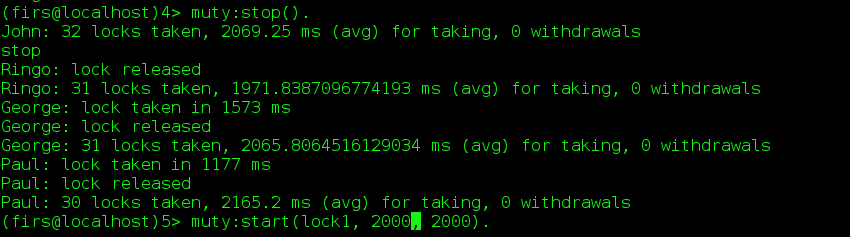
\includegraphics[width=1.0\textwidth]{figures/2000-2000lock1}
    \caption{Sleep 2000, Work 2000 \label{fig:2000-2000lock1}}    
\end{figure}


Es pot veure que l'execució és l'esperada. El \texttt{withdrawal} és de 8
segons, tal i com està per defecte. En la figure~\ref{fig:2000-2000lock1} es pot
veure que aquest valor està a zero per tots els clients. Per tant, no hi ha cap
d'ells que s'hagi vist obligat a rellançar la petició d'accés a regió crítica.

Donat que el temps de sleep és ''gran'' no es forcen locks. 

\subsubsection{Prova amb Sleep 20, Work 16000}

\begin{figure}[H]
	\centering
    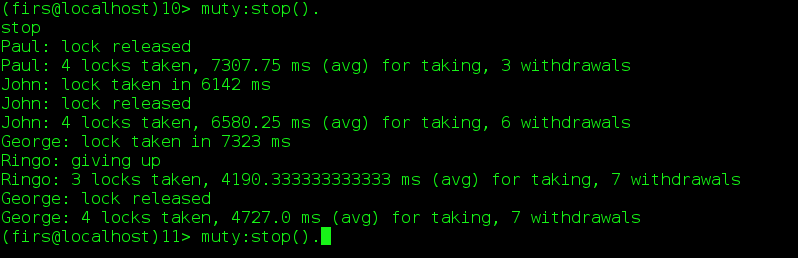
\includegraphics[width=1.0\textwidth]{figures/20-16000lock1}
    \caption{Sleep 20, Work 16000 \label{fig:20-16000lock1}}    
\end{figure}

En aquest experiment s'ha forçat que els workers sol·licitin accés a regió
crítica de manera molt freqüent, en proporció a la finestra de temps que un
worker necessita per executar-se.  
Es pot apreciar a la figure~\ref{fig:20-16000lock1} que el rendiment del sistema
baixa notòriament. El temps mig d'espera augmenta molt amb aquesta prova degut a
que hi ha molts intents d'accés a regió crítica no resolts. El paràmetre
\texttt{withdrawal} ha augmentat perquè hi ha molts processos que es veuen
forçats a fer el timeout i sol·licitar accés a regió crítica de nou.

\subsubsection{Prova amb Sleep 20, Work 20}

\begin{figure}[H]
	\centering
    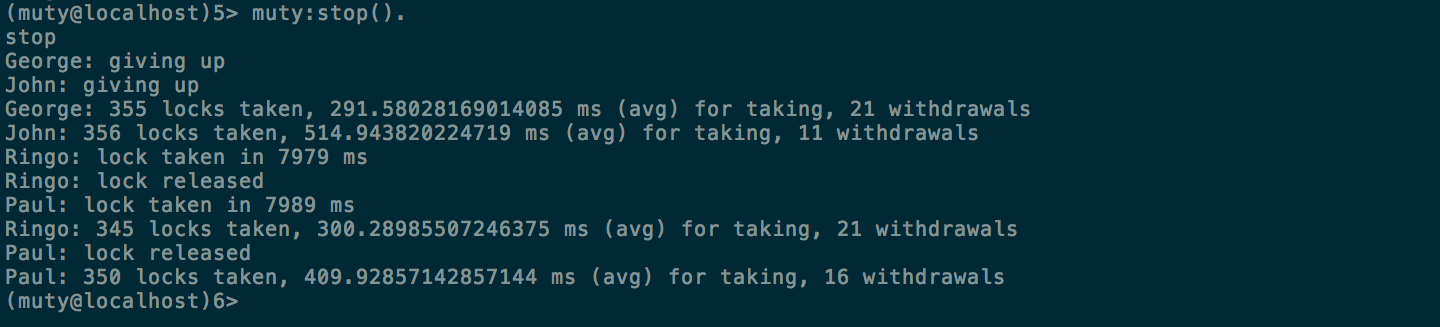
\includegraphics[width=1.0\textwidth]{figures/20-20lock1}
    \caption{Sleep 20, Work 20 \label{fig:20-20lock1}}    
\end{figure}

Per concloure les proves fetes sobre la implementació \textit{lock1} s'ha
estudiat el comportament amb valors de \texttt{Sleep} i \texttt{Work}
''petits''. En aquest experiment s'ha pogut veure que el sistema distribuit
pateix un deadlock. Tots els nodes executen la sol·licitud d'accés a les regions
crítiques respectivament al mateix temps. Això provoca que tots vegin que la
seva sol·licitud és la prioritària i per tant no validin la resta de requests.

\subsection{Lock2}

La segona implementació consisteix en solucionar els possibles deadlocks. Per
fer-ho s'ha utilitzat un sistema de prioritats a partir d'identificadors lògics
de node. El node més petit és el que té prioritat, alhora d'entrar a la regió
crítica, en cas d'empat. 

\subsection{Lock3}

\section{Preguntes directes}

% Try to answer all the open questions in the documentation. When possible, do
% experiments to support your answers.

\section{Opinió personal}


\end{document}

